%comment out for student version
\ifdefined\Student\relax\else\def\Teacher{}\fi

\documentclass[12pt,twoside,openright]{report}

\title{Activities for CS0}
\author{Chris Mayfield}
\date{Summer 2021}

%\ProvidesPackage{cspogil}

% fonts
\usepackage[utf8]{inputenc}
\usepackage[T1]{fontenc}
\usepackage{mathpazo}

% spacing
\usepackage[margin=2cm]{geometry}
\renewcommand{\arraystretch}{1.4}
\setlength{\parindent}{0pt}

% orphans and widows
\clubpenalty=10000
\widowpenalty=10000
\pagestyle{empty}

% figures and tables
\usepackage{graphicx}
\usepackage{multicol}
\usepackage{tabularx}
\usepackage{wrapfig}

% fixed-width columns
\usepackage{array}
\newcolumntype{L}[1]{>{\raggedright\let\newline\\\arraybackslash\hspace{0pt}}m{#1}}
\newcolumntype{C}[1]{>{\centering\let\newline\\\arraybackslash\hspace{0pt}}m{#1}}
\newcolumntype{R}[1]{>{\raggedleft\let\newline\\\arraybackslash\hspace{0pt}}m{#1}}

% include paths
\makeatletter
\def\input@path{{Models/}{../../Models/}}
\graphicspath{{Models/}{../../Models/}}
\makeatother

% colors
\usepackage[svgnames,table]{xcolor}
\definecolor{bgcolor}{HTML}{FAFAFA}
\definecolor{comment}{HTML}{007C00}
\definecolor{keyword}{HTML}{0000FF}
\definecolor{strings}{HTML}{B20000}

% table headers
\newcommand{\tr}{\bf\cellcolor{Yellow!10}}

% syntax highlighting
\usepackage{textcomp}
\usepackage{listings}
\lstset{
    basicstyle=\ttfamily\color{black},
    backgroundcolor=\color{bgcolor},
    numberstyle=\scriptsize\color{comment},
    commentstyle=\color{comment},
    keywordstyle=\color{keyword},
    stringstyle=\color{strings},
    columns=fullflexible,
    keepspaces=true,
    showlines=true,
    showstringspaces=false,
    upquote=true
}

% code environments
\newcommand{\java}[1]{\lstinline[language=java]{#1}}%[
\lstnewenvironment{javalst}{\lstset{language=java,backgroundcolor=}}{}
\lstnewenvironment{javabox}{\lstset{language=java,frame=single,numbers=left}\quote}{\endquote}

% PDF properties
\usepackage[pdftex]{hyperref}
\urlstyle{same}
\makeatletter
\hypersetup{
  pdftitle={\@title},
  pdfauthor={\@author},
  pdfsubject={\@date},
  pdfkeywords={},
  bookmarksopen=false,
  colorlinks=true,
  citecolor=black,
  filecolor=black,
  linkcolor=black,
  urlcolor=blue
}
\makeatother

% titles
\makeatletter
\renewcommand{\maketitle}{\begin{center}\LARGE\@title\end{center}}
\makeatother

% boxes [optional height]
\newcommand{\emptybox}[1][10em]{
\vspace{1em}
\begin{tabularx}{\linewidth}{|X|}
\hline\\[#1]\hline
\end{tabularx}}

% models
\newcommand{\model}[1]{\section{#1}\nopagebreak}
\renewcommand{\thesection}{Model~\arabic{section}}

% questions
\newcommand{\quest}[1]{\subsection*{Questions~ (#1)}}
\newcounter{question}
\newcommand{\Q}{\vspace{1em}\refstepcounter{question}\arabic{question}.~ }
\renewcommand{\thequestion}{\#\arabic{question}}

% sub-question lists
\usepackage{enumitem}
\setenumerate[1]{label=\alph*)}
\setlist{itemsep=1em,after=\vspace{1ex}}

% inline answers
\definecolor{answers}{HTML}{C0C0C0}
\newcommand{\ans}[1]{%
\ifdefined\Student
    \leavevmode\phantom{~~\textcolor{answers}{#1}}
\else
    ~~\textcolor{answers}{#1}
\fi}

% longer answers [optional height]
\newsavebox{\ansbox}
\newenvironment{answer}[1][4em]{
\nopagebreak
\begin{lrbox}{\ansbox}
\begin{minipage}[t][#1]{\linewidth}
\color{answers}
}{
\end{minipage}
\end{lrbox}
\ifdefined\Student
    \phantom{\usebox{\ansbox}}%
\else
    \usebox{\ansbox}%
\fi}


\usepackage{pdfpages}
\usepackage{pax}

% remove page numbers
%\makeatletter
%\let\ps@plain\ps@empty
%\makeatother

% dots in toc chapters
\usepackage{tocloft}
\renewcommand{\cftchapleader}{\cftdotfill{\cftdotsep}}

% include activity pdf
\newcommand{\act}[3]{
  \cleardoublepage\phantomsection
  \addcontentsline{toc}{chapter}{#2}
  \addtocontents{toc}{\nopagebreak\bigskip{#3}\par}
  \ifdefined\Teacher
    \includepdf[pages=-, pagecommand={}]{#1_Teacher.pdf}
  \else
    \includepdf[pages=-, pagecommand={}]{#1_Student.pdf}
  \fi
}

\begin{document}

\pagenumbering{roman}
\setcounter{page}{1}

\pdfbookmark{Title Page}{title}
\begin{titlepage}
\null\vfill
\centering


\includegraphics{../IntroCS.pdf}

\makeatletter

\vspace*{4em}
\huge \textbf{\@title}

\vspace*{2pt}
\ifdefined\Teacher
\color{DarkRed}
\Large \textbf{Instructor's Guide with Solutions}
\else
\color{ForestGreen}
\Large \textbf{Student Workbook}
\fi
\normalcolor

\vspace*{2em}
\large \@author

\vspace*{4pt}
\small With contributions from Helen Hu, \\ Clif Kussmaul, Mike Lam, and Greg Keim

\vspace*{2em}
\Large \@date

\makeatother

\normalsize

\vspace*{4em}

\includegraphics{../by-nc-sa.png}

\vspace*{1ex}
Copyright \textcopyright\ 2021.
This work is licensed under a Creative Commons Attribution-NonCommercial-ShareAlike 4.0 International License.

%\ifdefined\Teacher
%\vspace*{2em}
%
\includegraphics[height=4em]{Overleaf.png}
%
%\vspace*{1ex}
%Source documents available in Overleaf
%\fi

\vfill\null
\end{titlepage}

\cleardoublepage
\pdfbookmark{Preface}{pre}
\chapter*{Preface}
\thispagestyle{empty}

The activities in this collection have been designed for implementing Process Oriented Guided Inquiry Learning (POGIL) in Computer Science. POGIL is an evidence-based instructional strategy that helps students to construct their own knowledge and develop process skills. The activities generally follow a learning cycle of exploration, concept invention / term introduction, and application. Students work in small teams of 3-4 to discuss each model and answer the questions during class time. The instructor facilitates the process, creates opportunities for teams to report out, and offers additional guidance as needed. See \url{https://pogil.org/} for more information about POGIL and its effectiveness.

\bigskip

Students typically work together in the same team for multiple class periods (e.g., for an entire unit of the course). Each student should have an assigned role on the team, and the roles should rotate frequently (e.g, each week of the course). The \textit{Manager} (or Coordinator) keeps track of time and helps the team to stay on task. The \textit{Presenter} (or Spokesperson) speaks on behalf of the team when reporting out. The \textit{Recorder} (or Quality Control) reviews notes and helps the team reach consensus. The \textit{Reflector} (or Process Analyst) observes and comments on team dynamics. By taking on different roles at different times, more students have the opportunity to practice these skills.

\bigskip

Before each activity, the instructor should spend a minute or two providing context for how the topics relate to what was learned in previous classes. While students work, the instructor should circulate among the teams to monitor progress and provide assistance. Student teams should employ the instructor as a facilitator of learning rather than a source of information. The instructor should avoid giving or confirming answers to key questions. Teams should be invited periodically to report out to the whole class or to neighboring teams. It's unnecessary to report out every question.

\bigskip

Students should not view these activities as assignments to be completed individually. Rather, they are scripts that guide team discussion and inquiry during class time. Implementing the activities in this way is essential for students to develop process skills such as teamwork, critical thinking, problem solving, and interpersonal communication. Instructors should motivate students to capture key insights from the team discussion and not just passively write down answers to questions. The activity sheets are the student's notes for the day and should help them when studying for exams.

\bigskip

At the end of each activity, students should complete some type of assessment to demonstrate content knowledge and process skills. A generic \textit{Team Report} is included with this collection. Chapter 10 of the POGIL book (\url{https://pogil.org/curricular-materials/general-pogil-book}) has many additional suggestions for assessment. Instructors might also use prompts from the \textit{Instructor's Guide to POGIL} (pages 40--42 of \url{https://pcrest.com/research/POGIL_Instructor_Guide2014.pdf}). For more in-depth assessment of process skills, the ELIPSS project has rubrics (\url{https://elipss.com/process-skills.html}) that can be used both inside and outside of class.

\bigskip

If you have any feedback regarding these activities, please don't hesitate to contact me. I would love to hear how they worked in your classroom and am constantly looking for new ways to improve them.

\bigskip

% email link
\newcommand{\email}[1]{<\href{mailto:#1}{#1}>}

Chris Mayfield \email{mayfiecs@jmu.edu}


\cleardoublepage
\pdfbookmark{\contentsname}{toc}
\tableofcontents
\addtocontents{toc}{\protect\thispagestyle{empty}}

\clearpage\phantomsection
\addcontentsline{toc}{chapter}{Role Cards}
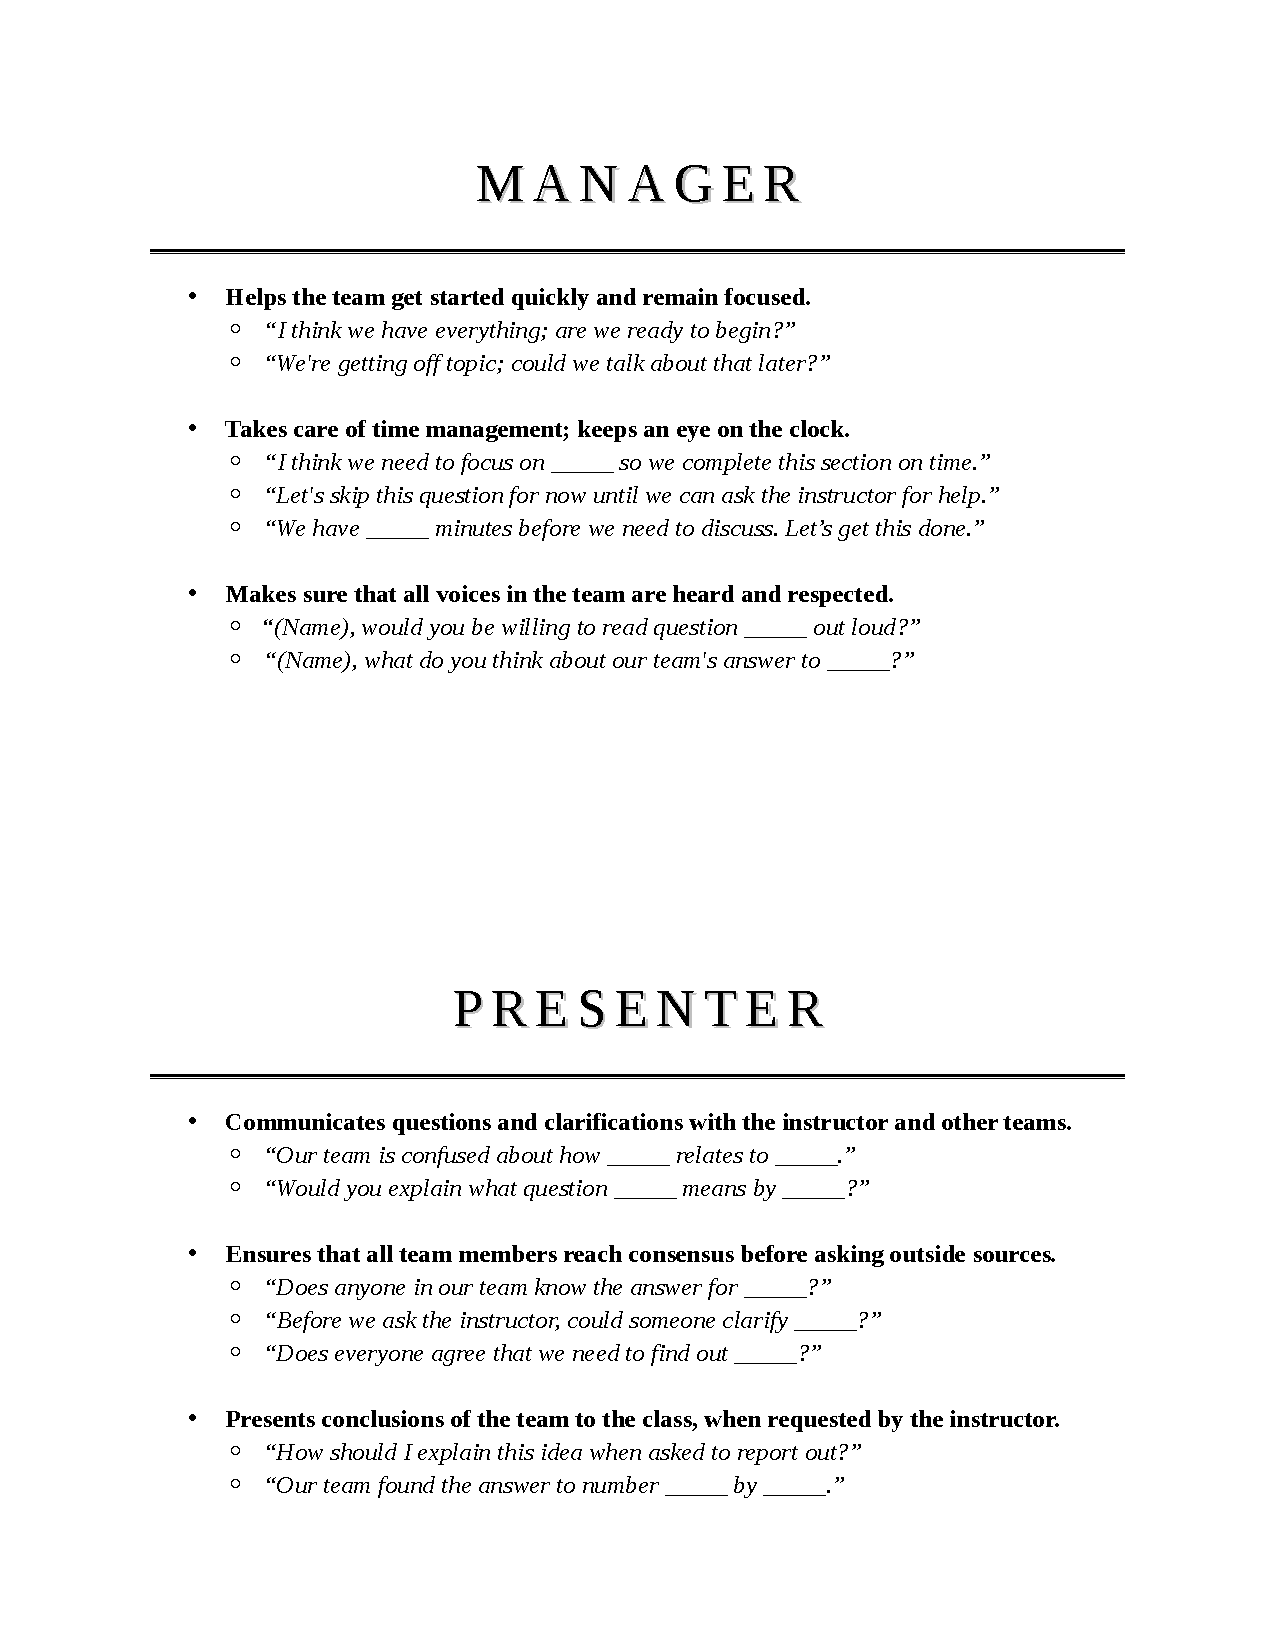
\includepdf[pages=-]{../Handouts/role-cards-appendix.pdf}

\clearpage\phantomsection
\addcontentsline{toc}{chapter}{Team Report}
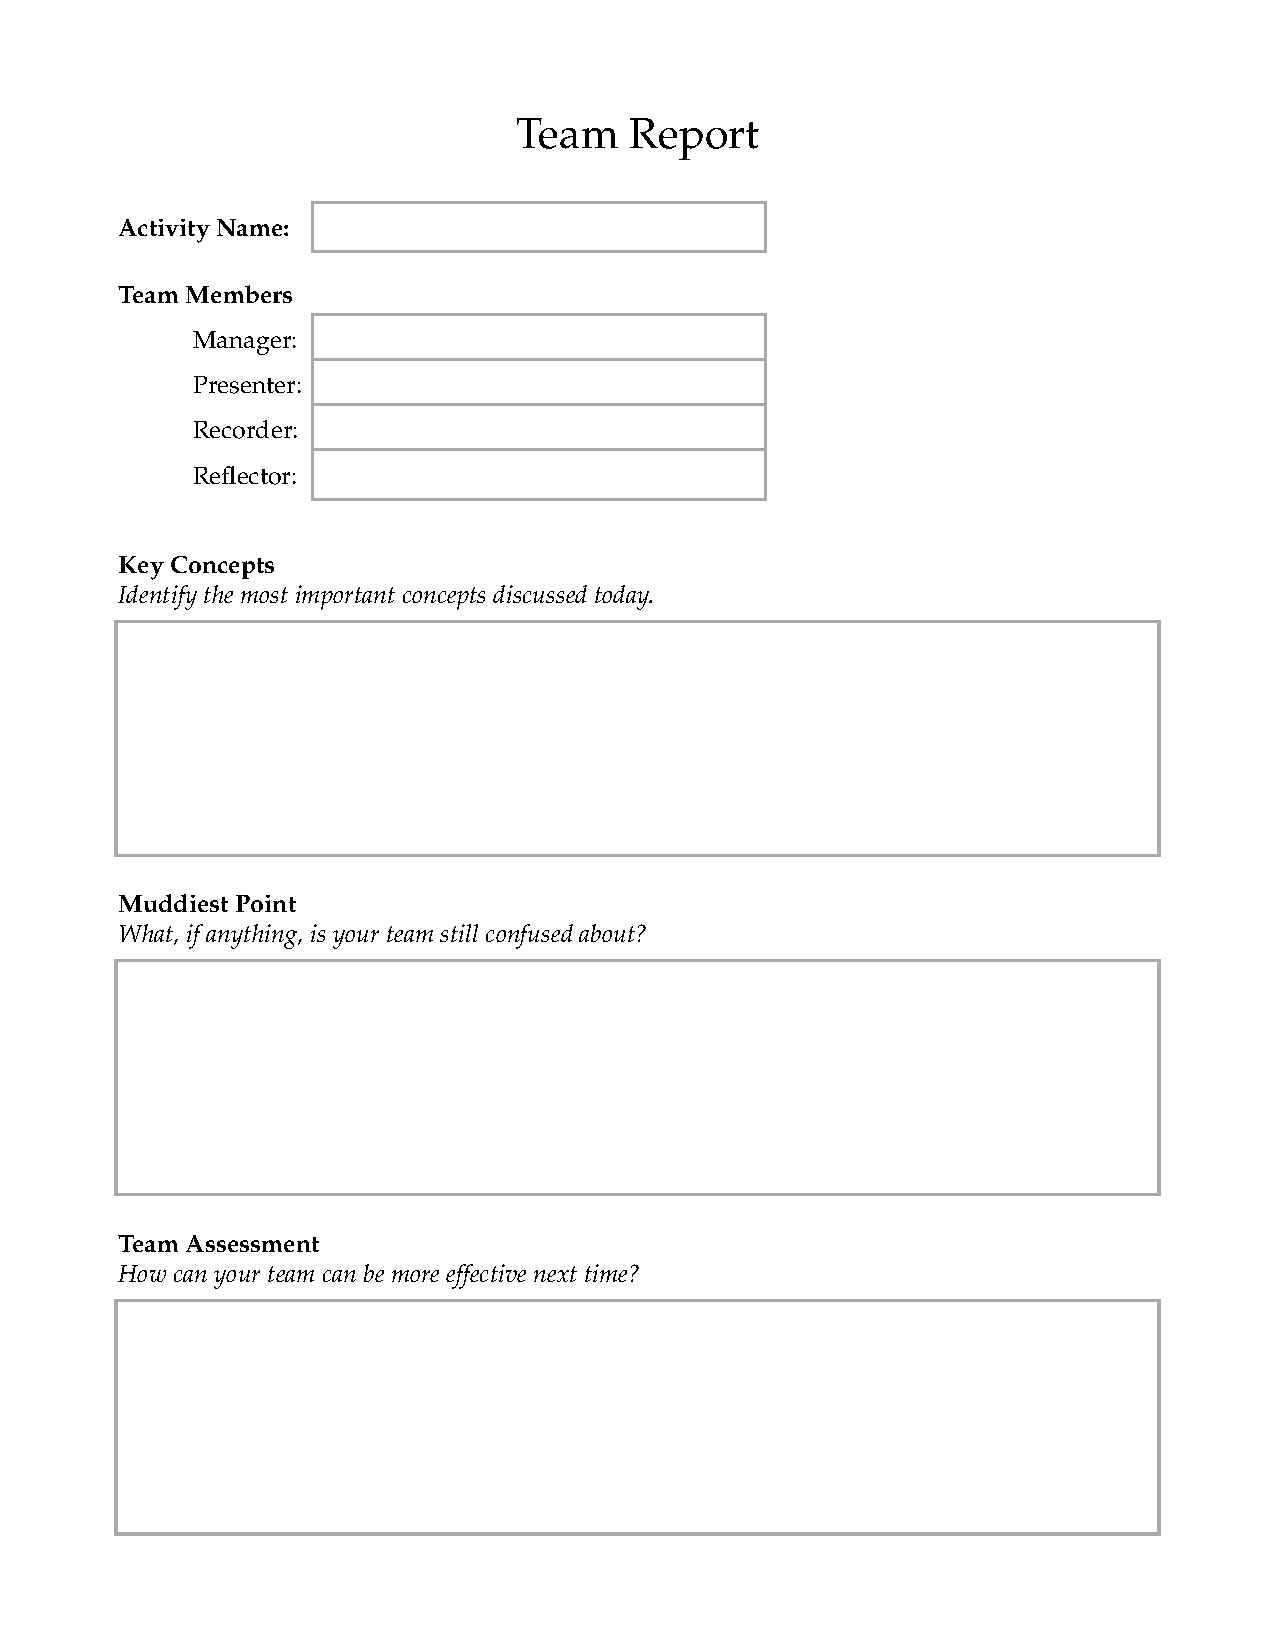
\includepdf[pages=-]{../Handouts/team-report.pdf}

\cleardoublepage
\pagestyle{plain}
\pagenumbering{arabic}
\setcounter{page}{1}

\renewcommand{\indent}{\hspace*{1.5em}}
\newcommand{\mod}[1]{\indent Model~#1~~}

%\addtocontents{toc}{\newpage}

\act{Act01/Act01-Algorithms}{Activity 1: Algorithms}{
\mod{1} Hi-Lo Game
}
\act{Act02/Act02-BitsBytes}{Activity 2: Bits and Bytes}{
\mod{1} Logic Gates \\
\mod{2} Binary Numbers
}
\act{Act03/Act03-Hardware}{Activity 3: Hardware}{
\mod{1} Computer Architecture \\
\mod{2} Machine Instructions
}
\act{Act04/Act04-Operating}{Activity 4: What is an OS?}{
\mod{1} Screenshots \\
\mod{2} Interactions
}
\act{Act05/Act05-Internet}{Activity 5: The Internet}{
\mod{1} How the Internet Works \\
\mod{2} Measuring Your Network
}
\act{Act06/Act06-Encryption}{Activity 6: Encryption}{
\mod{1} Random Substitution \\
\mod{2} Caesar Cipher \\
\mod{3} Vigenère Cipher
}
\act{Act07/Act07-HelloPython}{Activity 7: Hello, Python!}{
\mod{1} Using IDLE \\
\mod{2} Guessing Game
}
\act{Act08/Act08-Languages}{Activity 8: Programming Languages}{
\mod{1} Low-Level Languages \\
\mod{2} High-Level Languages
}
\act{Act09/Act09-LifeCycles}{Activity 9: Software Development}{
\mod{1} Finding \& Fixing Errors \\
\mod{2} The Waterfall Model \\
\mod{3} The Iterative Model
}
\act{Act10/Act10-DataStruct}{Activity 10: Data Structures}{
\mod{1} Array \\
\mod{2} Linked List
}
\act{Act11/Act11-Relational}{Activity 11: Relational Operations}{
\mod{1} Select and Project \\
\mod{2} Product and Join
}
\act{Act12/Act12-EightPuzzle}{Activity 12: Artificial Intelligence}{
\mod{1} The 8-Puzzle \\
\mod{2} Search Trees
}

%\cleardoublepage
%\thispagestyle{empty}
%\begin{center}
%\null\vfill
%\huge\bf Appendix
%\vfill\null
%\end{center}

\end{document}
